System test consist of 5 map of different sizes and complexity level. Each algorithm is tested with every map with the same positioning of the agents. Test time is defined as end end-to-end time, starting from test triggering in a backend and stopping when backend receives paths from all agents. More detailed information such as "test setup time", "communication time" and "algorithm calculation time" can be found in observability suite(grafana).

\subsection{System simulated in the cloud}
This system can be simulated both in a local environment as well as in cloud. Multiple agents can be created and connected to a system by spawning multiple kubernetes pods. This scenario is not taking into account communication delay as all containers are communicating in a local network(cluster network).

\subsection{Real system}
Small system composed of three external devices(rasperry pi) was created to showcase how real system would work. In each of devices agent container was deployed. On one of them there are map-servcie and broker containers. Scheme of the devices connection can be seen on diagram \ref{fig:cluster}.
\begin{figure}[H]
    \centering
    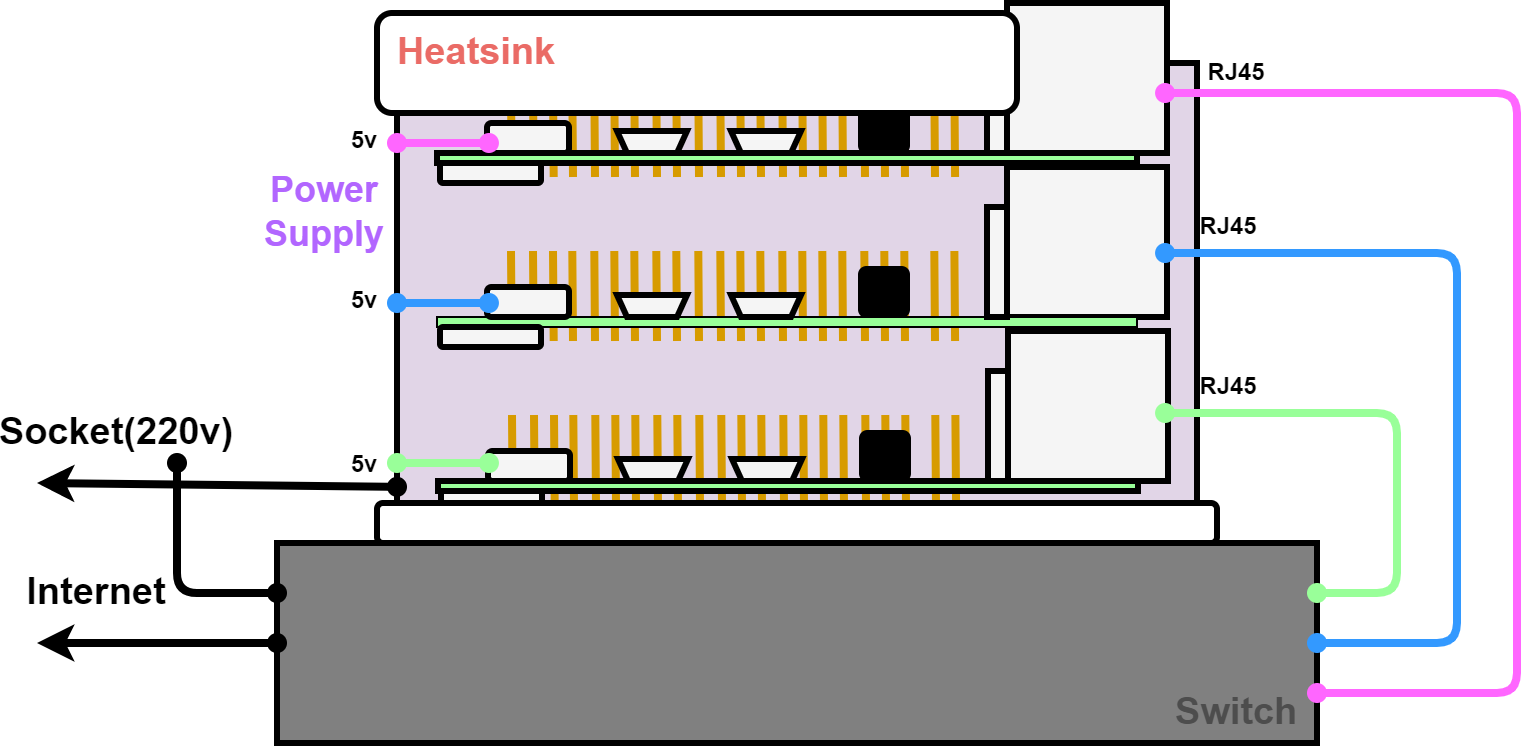
\includegraphics[width=0.8\textwidth]{pictures/cluster.png}
    \caption{ Real cluster }
    \label{fig:cluster}
\end{figure}

This setup resemble real-world scenario, with 3 robots(agents) and one server meant for deploying broker and communicating to the cloud. Agents has limited resources as Single Board Computer used for deployment only has 1GB of memory and Quad core Cortex-A72 1.5GHz processor\cite{rpi_specs}. For the purpose of the test computing power can also be throttled. Devices are connected to local network via internet switch. 

Challenging part was that those devices are using ARM architecture, therefore containers has to be rebuild to support this architecture. To ease a development struggle, azure devops agents were installed on the machines and Continous Integration pipeline was put in place, which rebuilds ARM images on every code change using locl machines as hosts and pushes them into image registry.Cloud part of the solution is deployed in okteto cloud and both parts are exchanging messages via mqtt brokers.

\subsection{System composed from virtual machines}
Another way of testing the system is to create set of virtual machines or containers locally and connect them to cloud system. Benefits of this approach are that this setup is easier to maintain, it supports x86 architecture and is easily extensible, as for spawning more agent there is no additional hardware needed. Resource limits can also be implemented both in case of container and virtual machines. Those entities has to be put in same virtual network to enable communication between simulated machines.